\section{Method}
\label{sec:method}

Assuming $p$ variants and a dichotomous phenotype of $n$ subjects was acquired.
For the $ith$ subjects lets denote $\bm{G_i} = (G_{i1}, G_{i2},\ldots , G_{ip})$ and $y_i$ as the genotype as well as the phenotype respectively.
Further I assumed an additive genetic model and let $G_{ip} = 0, 1, 2$ represent the number of rare alleles at variant $p$.  

One can then calculate the \acrfull{ECDF} for both cases ($F_{A(G)}$) and controls ($F_{U(G)}$) or any other dichotomous phenotype.
The ecdf is a monotonic step function, increasing from $0$ at the first position of the gene, to $1$ at the last position of the gene.
For $p$ rare variants occurring at positions  $G_{i1}, G_{i2}, \ldots, G_{ip}$, the empirical distribution function of $G$ is given by

\begin{equation}
  F(x) = \frac{1}{p}\sum^p_{i=1}I(X_i \leq x)
\end{equation}

in which $I(x)$ is the indicator function for a fixed given variant $x$.
The KS statistic $K$ is defined as the supremum of the absolute difference between the two empirical distribution functions.

\begin{equation}
	K_{KS} = \sup_x | F_A(x) - F_U(x) |
\end{equation}

While the KS test is distribution free when $F$ is continuous, this is not the case with discrete data, such as allele count.
Indeed, application of the Kolmogorov distribution to obtain critical values for $K$ for discrete data yields conservative estimates~\cite{Walsh1963,Conover1972}. 
\citet{Conover1972} proposed an alternative way to obtain critical values given a hypothesized discrete distribution function.
However, this approach is not feasible with samples sizes $>30$.
Therefore, I applied a permutation based approach to estimate p-values as 
\begin{equation}
  p_{per} = \frac{\sum^b_{b=1} I(K_b \geq k)+1}{b+1}
\end{equation}
in which $K_b$ is the test statistic of the $b^{th}$ permuted sample.

\subsection{Omnibus Test for KS and Burden}
\label{sub:omnibus_test_for_ks_and_burden}

The KS test makes the strong assumption that in a given genomic region only a certain causal cluster of rare variants are related to the phenotype in question.
This assumption does not contradict that of the burden test which assumes that all variants under investigation have the same direction of effect and can be seen as two sides of the same coin.
Thus it might be desirable to combine the two test statistics in order to obtain a combined test statistic, given that those test statistics are independent.

I define the test statistic of the burden test as 
\begin{equation}\label{eq:burden_simple}
  K_{Burden} = (\sum^p_{i=1} (\bm{y}-\bar{y}) \times \bm{G_i})^2
\end{equation}
This is equivalent to the form described in Section~\ref{sub:burden_test}.

One can combine the two tests by Fischer's method 
\begin{equation}
	\chi^2_4 \sim - 2 (\ln(p_{KS}) + \ln(p_{Burden}))
\end{equation}
in which the test statistic $\chi^2$ follows a $\chi^2$-distribution with $4$ degrees of freedom.
I have choose to call this combined test KS-Burden.

Implementation of the KS, Burden and KS-Burden was done in C++ and can be found at \url{https://github.com/rmporsch/ksburden}.
This repository also includes associated scripts and programs to repeated simulations described within this manuscript.

\subsection{Simulation Study}
\label{sub:simulation_study}

In contrast to most previous simulation studies investigating the statistical properties of rare variant association tests I made use of actual sequencing data.
Thus, genotypes were not simulated but acquired from previous association studies.
The main aim of using real data is to accurately reflect the diversity of genes within the human genome as well as limitations commonly encountered in sequencing based studies.
Most gene based tests are confronted with a variety of small and medium gene lengths which is often not reflected in the original power estimations.
Hence I will make use of a large sequenced sample to investigate the statistical properties of the KS and KS-Burden test.

\subsubsection{The Seed population: The Hirschsprung data}
\label{ssub:The_Seed_population:_The_Hirschsprung_data}

Hirschsprung's disease (HSCR) is a rare congenital disorder occurring in about one of $5,000$ births~\cite{Amiel2001}.
The here used sample contains 464 cases as well as 498 controls analyzed by whole genome sequencing (36.6X median read depth).
All patients are sporadic cases with known family history of HSCR and were recruited in China ($n=341$) and Hanoi, Vietnam ($n=102$).
Controls were obtained from same or nearby cities in order to match the subpopulation of patients.
Samples were excluded due to failure in heterozygosity, gender accordance, duplications and relatedness.
Ethical outliers were removed by PCA resulting in a final set of 443 cases and 493 controls.
Further, genotype level quality control was applied with KGGseq~\cite{Li2012b} and genotypes with quality less than 20 ($GQ<20$) or covered by less than 8 reads ($DP<8$) were excluded.
In addition, variants with call rate $<0.9$ or those violating Hardy-Weinberg equilibrium ($P<1\times 10^{-5}$) were removed.
This resulted in a final call set of 33.5 millions (M) SNVs and 3.3M indels, the majority of which are novel (61.5\% for SNVs and 68.7\% for indels). 

Variants were then annotated for protein functions against the RefSeq gene annotations as well as population frequencies (1000 Genomes Project phase 3, ExAC and ESP).
Only non synonymous exonic variants (frameshift, nonframeshift, stopgain, missense, startloss, stoploss, splicing) with an MAF $\leq 1\%$ were included in the simulations. 
Overall frequency of rare non synonymous mutations are displayed in Figure~\ref{fig:num_var} and show great variations.
The number of rare variants per gene ranged from $3$ to $491$ with a median of $5$.

\begin{figure}[htpb]
  \centering
  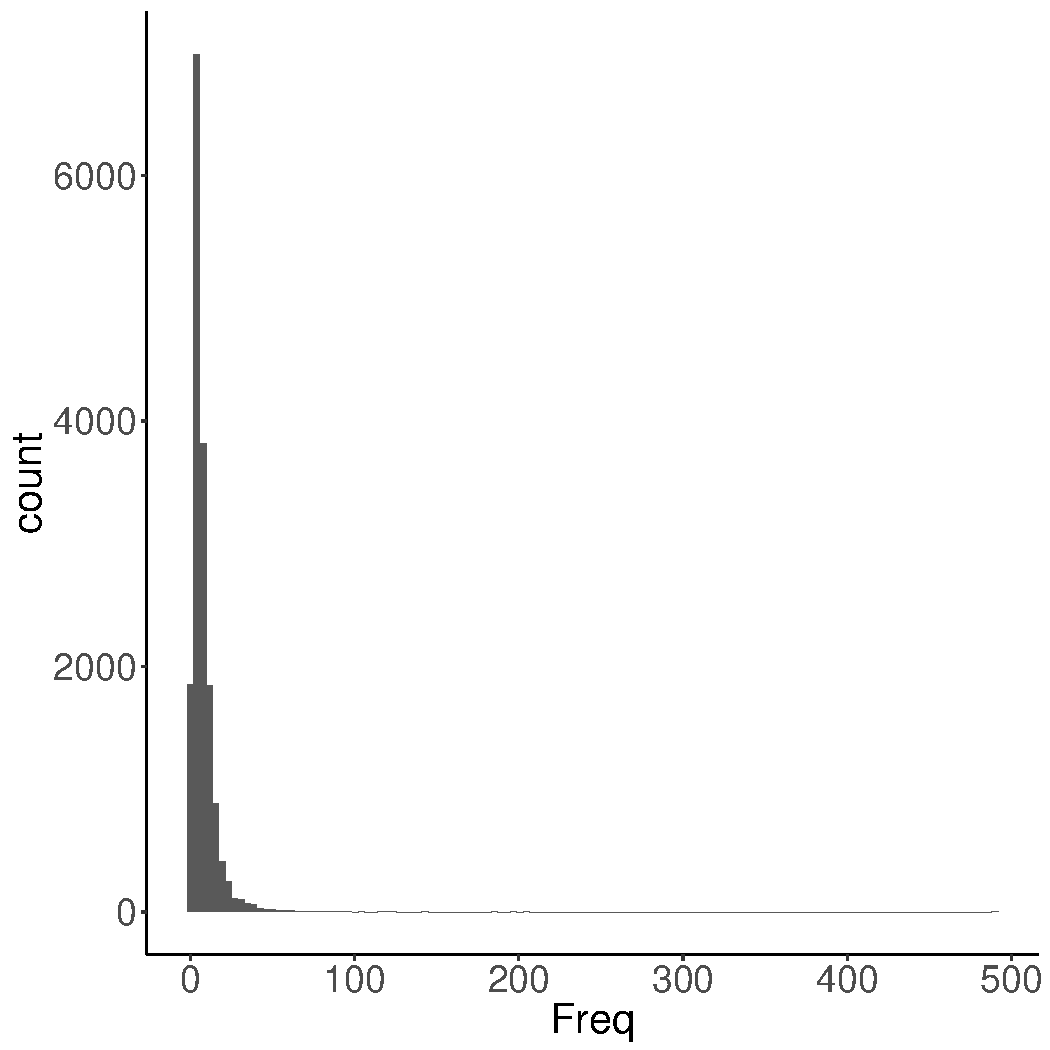
\includegraphics[width=0.5\linewidth]{ksburden/figures/number_var_genes.pdf}
  \caption[Frequency of rare variants]{Overall frequency of rare non-synonymous mutations.}\label{fig:num_var}
\end{figure}

\subsubsection{Simulation Framework}
\label{ssub:Simulation_Framework}

From the set of $16,510$ genes I selected 50 genes at random which had at least 3 or more rare variants. 
Mutation were defined as rare if the Minor Allele Frequency (MAF) was below or equal 1\%. 
Within $p$ rare variants of a gene I assigned causal status to $p_1 \ldots p_t$ positions, in which $t$ represents the total number of causal variants.
For simplicity I assigned the causal cluster at the beginning of the gene.
Within these simulations I gradually increased the size of the causal cluster to eventually cover the whole gene. 

The phenotype was simulated via a liability threshold model.
Hence the phenotype $Y_i$ of the $i^{th}$ subject was generated via
$Y = G\times E' + \epsilon$
in which $G$ is the standardized genotype matrix of $n=1000$ subjects with $p$ variants.
$E$ is the effect size vector of size $1\times p$ and $\epsilon$ is a standard normal distributed error term with a mean of $0$ and a standard deviation of $\sqrt{1-h^2}$, in which $h^2$ is the assumed heritability or the genetic effect on the liability distribution.
The effect $h$ was uniformly distributed across all causal variants.
I assigned case status for each subjects whose $Y_i$ is above a certain liability threshold $q$.
Any subject above $q$ was assigned case status, while the remaining subjects were deemed to be controls.
This process was repeated until $500$ cases and an equal number of controls were collected.

\subsubsection{Application of the KS-Burden}
\label{ssub:Application_of_the_KS-Burden}

The KS-Burden test was further applied to the UK BioBank to investigate distributional differences of rare variants between aggressive and non aggressive individuals.
As described in the previous chapter the UK BioBank is a chip-array data set.
Commonly genotyped data is not applicable for rare variant testing due to the low imputation quality of low frequency variants.
However, given a very large sample size, imputation quality is gradually improving thus allowing the investigations of rare variants.
Indeed, the UK BioBank is with over $150,000$ samples relatively large.
As can be seen in Figure~\ref{fig:imputation}, imputation quality is acceptable for variants with a frequency between 1\% and 0.1\%, given the commonly used quality score cut-off of $0.2$.
Therefore providing sufficient high quality variants to investigate potential distributional differences.

Similar quality control was applied as in previuos described usages of the UKB\@.
Basic quality control and imputation was performed central with the UKB\@.
Participants of non-caucasion ethnicity were excluded, as determined by a k-mean cluster of the first 3 principle components.
Variants which whose missing call rate did exceed 10\%, those which have an information score less than $0.2$, as well as those with minor allele frequency greater than $1\%$ and those lower then $0.1\%$ were excluded.
Further variants which did not pass a Hardy-Weinberg equilibrium test threshold of $1\times10^{-9}$ were also removed from the analysis.

Annotation of variants was done with KGGseq~\cite{Li2012b}
Only non synonymous exonic variants (frameshift, nonframeshift, stopgain, missense, startloss, stoploss, splicing) were included (RefSeq gene annotations).
In addition, genes with less or equal than $3$ variants were excluded from the analysis.
This resulted in $16,709$ variants distributed across $3,481$ genes.

\begin{figure}[htpb]
  \centering
  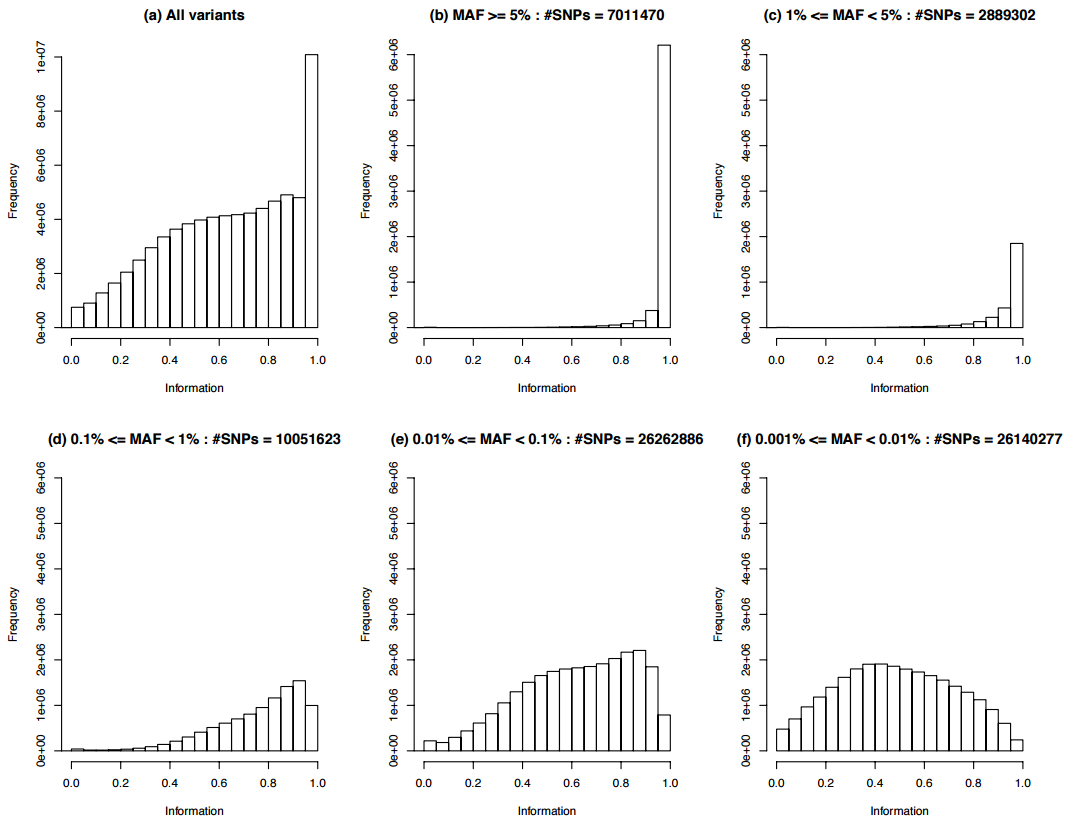
\includegraphics[width=0.8\linewidth]{ksburden/figures/imputation_qc.png}
  \caption[Imputation Quality]{Imputation Quality of the UK BioBank~\cite{Marchini2015}}\label{fig:imputation}
\end{figure}
